\subsection{Исследование системы с пропорциональным регулятором}\label{title:PR}
Составим систему
дифференциальных уравнений в операторной форме  для математического описания системы с пропорциональным регулятором 
относительно отклонения $x$.
\begin{figure}[!h]\centering
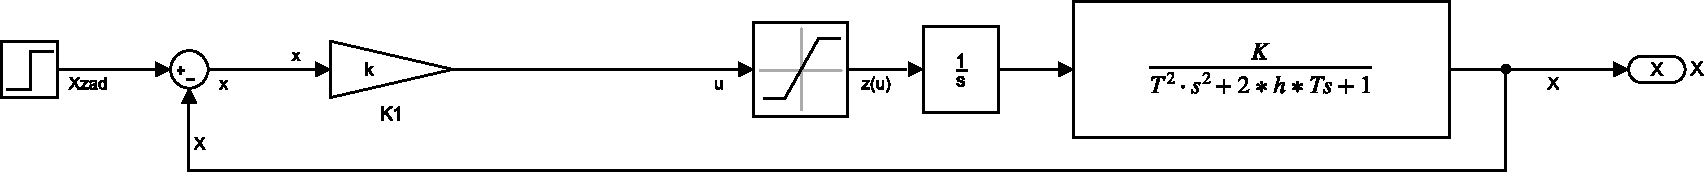
\includegraphics[width=1.0\linewidth]{images/sim_P}
\caption{СС замкнутой системы с пропорциональным регулятором.}\label{fig:sim_P}
\end{figure}
По СС замкнутой системы на рис.\ref{fig:sim_P} составим уравнения \eqref{eq:control_sys}.
\begin{equation}
    \begin{aligned} \label{eq:control_sys}
       x&=X_{zad}-X & X&=\cfrac{3\,z(u)}{Q(p)}\\
       Q(p)&=p\,\left(81\,p^2+108\,p+1\right)&Q(p)\,x&=Q(p)\,X_{zad}-3z(u)\\
    \end{aligned}
\end{equation}
Исследуем собственные свойства системы, т.е. считаем $X_{zad}=0$.
 Учтём, что мы имеем пропорциональный регулятор, т.е. $u=k_1\,x$, получаем уравнение
 \eqref{eq:con_sys1}
.
\begin{equation} \label{eq:con_sys1}
Q(p)\,x=-3\,z(k_1\,x)
\end{equation}
Далее раскроем функцию $z(u)$ и получим систему \eqref{eq:con_sys2}.
\begin{equation}
    \left\{
    \begin{aligned} \label{eq:con_sys2}
       p\,\left(81\,p^2+108\,p+1\right)\,x&=-3\,k_1\,x&&, \text{ если}|k_1\,x|\le 0.6\\
       p\,\left(81\,p^2+108\,p+1\right)\,x&=-1.8\,\mathrm{sign}\left(k_1\,x\right)&&, \text{ если}|k_1\,x|> 0.6\\
    \end{aligned}
    \right.
\end{equation}
Отсюда ХП замкнутой системы при $k_1\,x\le0.6$ \eqref{eq:key4}.
\begin{equation} \label{eq:key4}
D(p)=\left(81\,p^3+108\,p^2+p+3\,k_1\right)
\end{equation}
При $|k_1\,x|>0.6$ линейная обратная связь отсутствует и движение в ней определяется свойствами управляемого объекта, при условии, что на его вход подаётся постоянное по значению воздействие. При $|k_1\,x|\le0.6$ движение описывается линейным дифференциальным уравнением. Неустойчивость системы может быть вызвана:
\begin{enumerate}
\item 
Неустойчивостью линейной системы.
\item 
Неустойчивостью, вызванной релейным режимом работы при $|k_1\,x|\hm{>}0.6$.
\end{enumerate}

Определение предельного значения по критерию Гурвица:

$a_0=81,a_1=108,a_2=1,a_3=3\,k_1$
\begin{equation} \label{eq:key5}
a_1\.a_2-a_0\,a_3\ge0
\end{equation}
\begin{equation} \label{eq:sys_ust}
0\le k_1\le 0.444 \text{ --- для асимптотической устойчивости.}
\end{equation}
$k_1=0.444$ --- граница устойчивости колебательного типа. 
\begin{figure}[!h]\centering
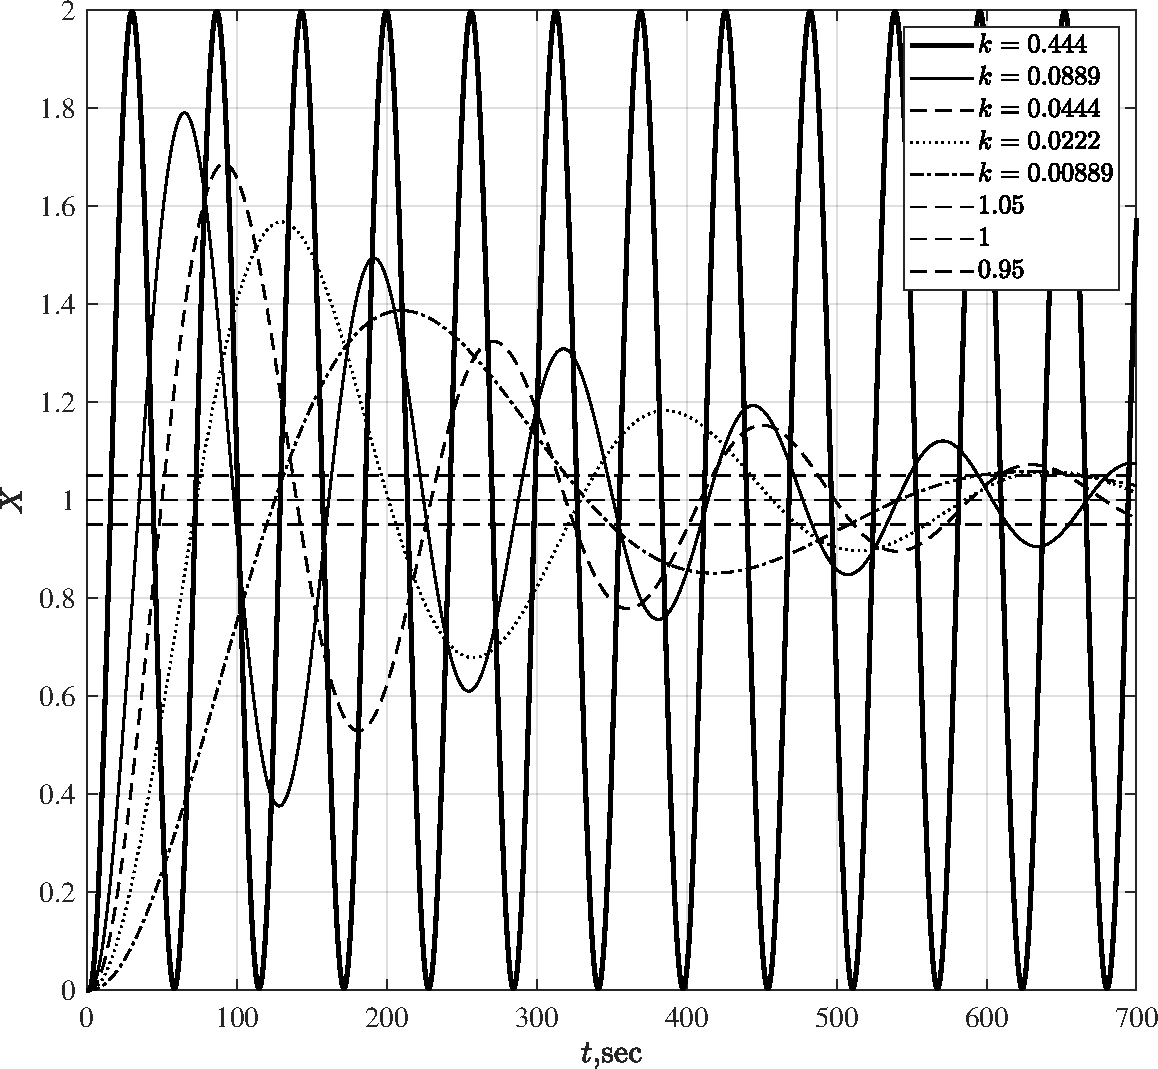
\includegraphics[width=1.0\linewidth]{images/P_sys}
\caption{ Графики изменения выходной переменной $X$ для разных $k$.}\label{fig:P_sys}
\end{figure}

Оценим ПХ регулируемой переменной при различных значениях $k$ для устойчивых режимов на рис.\ref{fig:P_sys}. Как видим при критическом значении $k_1$ появляются незатухающие колебания. При уменьшении $k$ значение показателя колебательности становится меньше.

Для повышения быстродействия нужно увеличить коэффициент передачи, но это ведёт к неустойчивости системы.
